\subsection{Ocular Artifact Correction}
We adapt the  Ocular Artifact Correction (OACL) technique developed in (add reference) for multi-class datasets. The OACL method consists of two parts. First, we analyse the raw EEG signals to obtain the artifact signals, representing the parts of the raw signal that was determined to be noise. Then we find the filtering parameter of each the artifact signal, which determines "how much" of each signal that should be removed from the raw signal. 

Let $x = \{s_0, ...,s_n\}$ where $s_t \in \mathbb{R}_{\geq 0}$ denote the raw EEG data for some arbitrary channel. For simplicity, we can interpret $x$ as a function $x : \mathbb{N}_{\geq 0} \rightarrow \mathbb{R}_{\geq 0}$ where $x(t)$ denotes the amplitude of $x$ at time $t$. 
% This file was created by matplotlib2tikz v0.5.7.
% The lastest updates can be retrieved from
% 
% https://github.com/nschloe/matplotlib2tikz
% 
% where you can also submit bug reports and leavecomments.
% 
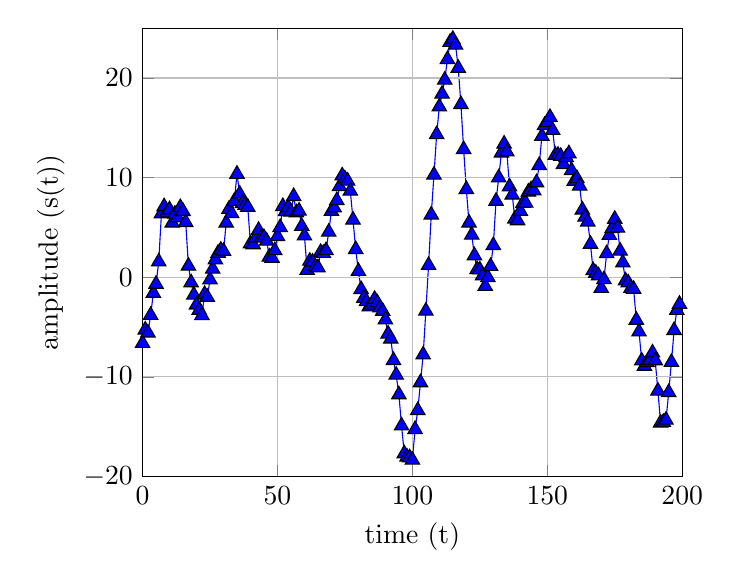
\begin{tikzpicture}

\begin{axis}[
xlabel={time (t)},
ylabel={amplitude (s(t))},
xmin=0, xmax=200,
ymin=-20, ymax=25,
axis on top,
xmajorgrids,
ymajorgrids
]
\addplot [blue, mark=triangle*, mark size=3, mark options={solid,draw=black}]
table {%
0 -6.62109375
1 -5.2734375
2 -5.576171875
3 -3.80859375
4 -1.591796875
5 -0.68359375
6 1.5625
7 6.396484375
8 7.099609375
9 6.474609375
10 6.796875
11 5.458984375
12 6.357421875
13 5.986328125
14 7.01171875
15 6.62109375
16 5.517578125
17 1.142578125
18 -0.537109375
19 -1.77734375
20 -2.763671875
21 -3.291015625
22 -3.828125
23 -1.69921875
24 -1.9921875
25 -0.244140625
26 0.830078125
27 1.767578125
28 2.431640625
29 2.724609375
30 2.626953125
31 5.458984375
32 6.826171875
33 6.416015625
34 7.63671875
35 10.361328125
36 8.369140625
37 7.421875
38 7.236328125
39 7.041015625
40 3.37890625
41 3.28125
42 3.974609375
43 4.7265625
44 3.96484375
45 3.994140625
46 3.642578125
47 2.05078125
48 1.923828125
49 2.685546875
50 4.111328125
51 5.009765625
52 7.119140625
53 6.611328125
54 7.001953125
55 6.572265625
56 8.125
57 6.494140625
58 6.66015625
59 5.126953125
60 4.169921875
61 0.712890625
62 1.630859375
63 1.533203125
64 1.0546875
65 0.9765625
66 2.509765625
67 2.412109375
68 2.685546875
69 4.541015625
70 6.640625
71 6.9921875
72 7.71484375
73 9.111328125
74 10.1953125
75 9.892578125
76 9.66796875
77 8.662109375
78 5.76171875
79 2.802734375
80 0.60546875
81 -1.2109375
82 -2.099609375
83 -2.431640625
84 -2.958984375
85 -2.783203125
86 -2.197265625
87 -2.548828125
88 -3.056640625
89 -3.3984375
90 -4.2578125
91 -5.68359375
92 -6.181640625
93 -8.33984375
94 -9.8046875
95 -11.77734375
96 -14.90234375
97 -17.6953125
98 -18.037109375
99 -18.095703125
100 -18.33984375
101 -15.263671875
102 -13.359375
103 -10.56640625
104 -7.7734375
105 -3.37890625
106 1.2109375
107 6.26953125
108 10.2734375
109 14.3359375
110 17.119140625
111 18.3984375
112 19.8046875
113 21.875
114 23.603515625
115 23.896484375
116 23.3203125
117 20.99609375
118 17.353515625
119 12.841796875
120 8.828125
121 5.46875
122 4.248046875
123 2.177734375
124 0.791015625
125 0.751953125
126 0.15625
127 -0.8984375
128 -0.01953125
129 1.103515625
130 3.203125
131 7.646484375
132 10
133 12.490234375
134 13.388671875
135 12.59765625
136 9.091796875
137 8.271484375
138 5.869140625
139 5.693359375
140 6.640625
141 7.44140625
142 7.4609375
143 8.57421875
144 8.798828125
145 8.69140625
146 9.501953125
147 11.240234375
148 14.169921875
149 15.25390625
150 15.556640625
151 16.064453125
152 14.755859375
153 12.265625
154 12.265625
155 12.1484375
156 11.337890625
157 12.03125
158 12.412109375
159 10.72265625
160 9.658203125
161 9.912109375
162 9.169921875
163 6.767578125
164 6.0546875
165 5.56640625
166 3.330078125
167 0.68359375
168 0.419921875
169 0.166015625
170 -1.09375
171 -0.224609375
172 2.3828125
173 4.228515625
174 4.892578125
175 5.83984375
176 4.9609375
177 2.646484375
178 1.455078125
179 -0.341796875
180 -0.546875
181 -1.103515625
182 -1.19140625
183 -4.296875
184 -5.46875
185 -8.37890625
186 -8.916015625
187 -8.544921875
188 -8.33984375
189 -7.578125
190 -8.359375
191 -11.40625
192 -14.609375
193 -14.55078125
194 -14.326171875
195 -11.552734375
196 -8.525390625
197 -5.322265625
198 -3.310546875
199 -2.6953125
};
\end{axis}

\end{tikzpicture}
From $x(t)$ we perform all steps in artifact detection and removal.

%Let $t \in \mathbb{N}_{\geq 0}$ be the time of a EEG sample, then $x(t)$ denotes the amplitude measured at time $t$, that is, $x(t)$ denotes the raw EEG signal for some channel.

\subsubsection{Artifact Detection}
The goal of artifact detection is to find some artifact signal $a(t)$ from $x(t)$ that represents which parts of $x(t)$ that are noise. Before finding the artifact signal $s(t)$, we first obtain a smoothed signal by applying a \emph{moving average filter} to $x(t)$. A moving average filter at time t, is computed as the average of $\frac{m}{2}$ samples on either side of the tth sample:
\begin{equation}
\label{eq:movavg}
s(t) = \frac{1}{m}\sum_{t-\frac{m}{2}}^{t+\frac{m}{2}}x(t)
\end{equation}
where $m$ is the number of neighboring points used.

From the smoothed signal $s(t)$ OACL finds the changes in amplitude between the samples, which could indicate eye movement. Therefore, we proceed by computing the relative heights between samples as the maximal difference in amplitude between a sample at time $t$ and its neighboring samples.
\begin{equation}
\label{eq:relheights}
\Delta (t) = max(|x(t)-x(t-1)|,|x(t+1) - x(t)|)
\end{equation}
Now, we want to have some measure of what an artifact signal looks like. \citet{li2015ocular} found by inspection that ocular artifacts generally occur with sudden changes in amplitude ($\Delta$) between $[30\mu V-50\mu V]$ and $[70\mu V-150\mu V]$. The problem with this approach is, that it does not generalize to data collected using different setups for the EEG measurement. For this reason, we automatically estimate the ranges by considering them parameters to be optimized through Bayesian Optimization.
For now, assume that we have some arbitrary ranges
\begin{equation}
\label{eq:ranges}
R=[l, u] \quad  l,u \in \mathbb{N}_{\geq 0}
\end{equation}
then we can find the points in time where $\Delta (t)$  lies in the range $R$:
\begin{equation}
\label{eq:peaks}
P = \{t \quad | \quad \frac{m}{2} < t < n-\frac{m}{2} \quad \textnormal{and} \quad l < \Delta (t) < u\}
\end{equation}
where $P$ is the indexes of the samples of the smoothed signal, where a change in amplitude lies within the range that characterizes an ocular artifact.

We now have the peaks of the ocular artifacts in $s(t)$, but we still need all of the artifact before we can correct it. The approach in the OACL method is to define the artifact to be from the closest zero point to the peak, before the peak, to the closest zero point after the peak. We can now find the artifact signal 
\begin{equation}
\label{eq:artifactsignal}
a(t) =
\begin{cases}
s(t)      & \quad \text{if } z_b \leq t < z_a\\
0  & \quad \text{otherwise}\\
\end{cases}
\end{equation}
where $z_b, z_a$ are the zero points after and before respectively. The concept of zero points of an artifact are illustrated in figure (todo: make figure).

Recalling that we can use an arbitrary number of ranges in \ref{eq:ranges}, we obtain the set of artifact signals for a single channel of a single trial as:
\begin{equation}
A(t)=  \begin{pmatrix}
a_1(t) \\
a_2(t) \\
\vdots  \\
a_n(t) 
\end{pmatrix}
\end{equation}
The idea behind this, is that different types of artifacts can be found by using different kinds of ranges. 
\subsubsection{Artifact Removal}
Explain how we use the artifact signals to remove artifacts from the eeg signal.